\documentclass[12pt,a4paper]{article}
\usepackage{header} % Use the provided header format
\usepackage[utf8]{inputenc}
\usepackage[T5]{fontenc}
\usepackage[vietnamese,english]{babel}

% ---------------------------------------------------------------
% Helpers for this report
% ---------------------------------------------------------------
% Origin marker:  \org{3}  ->  3 with an up-arrow underneath
\newcommand{\org}[1]{\underset{\uparrow}{#1}}

% Reserved (dashed) box for parts that are written by other members.
% Usage: \writespace[height]{hint text}
\newcommand{\writespace}[2][4cm]{%
  \begin{tcolorbox}[enhanced, frame hidden, colback=gray!4,
      borderline={0.6pt}{0pt}{gray!70, dashed},
      height=#1, valign=center, halign=center,
      fontupper=\itshape\small\color{gray}]
    #2
  \end{tcolorbox}}

% Scilab code listing from a file
\newcommand{\scilabfile}[2]{%
  \lstinputlisting[language=Scilab, caption={#2}]{#1}}

\begin{document}

\begin{center}
    \textbf{Digital Signal Processing \hfill HK261 \hfill CO2036}\\[2cm]

    \huge\textbf{DIGITAL SIGNAL PROCESSING LAB REPORT}\\[0.5cm]
    \Large\textbf{Lab 3 -- Script Functions for Discrete-Time Signals}\\[1cm]

    \large Âu Lê Quang Trí - Student ID: 2453300\\[0.5cm]
    \large Nguyễn Lê Khải Tú - Student ID: 2453384\\[0.5cm]
    % \large <Member 3> - Student ID: <ID>\\[0.5cm]
    % \large <Member 4> - Student ID: <ID>\\[0.5cm]
    \vspace{0.5cm}

    \large \today\\[2cm]
\end{center}

\section*{Overview}
This report presents the results of Lab 3 of the Digital Signal Processing laboratory. In this lab, the basic time-domain operations on discrete-time signals (delay, advance, folding, addition, multiplication and convolution) are implemented as reusable \textbf{Scilab script functions}. Every function receives a signal as a pair (\texttt{vector}, \texttt{origin position}), returns the resulting signal in the same format and graphically displays the input(s) and output in a single figure. The report also covers the additional exercises 2.1, 2.2, 2.4 and 2.6 of the reference document, both theoretically and practically on Scilab.

\begin{table}[H]
    \centering
    \caption{Content of the report}
    \begin{tabular}{|l|l|c|}
        \hline
        \rowcolor{headergray}\textbf{Part} & \textbf{Content} & \textbf{Section} \\ \hline
        Exercise 1 & \texttt{delay} -- $y(n)=x(n-k)$                   & \ref{sec:ex1} \\ \hline
        Exercise 2 & \texttt{advance} -- $y(n)=x(n+k)$                 & \ref{sec:ex2} \\ \hline
        Exercise 3 & \texttt{fold} -- $y(n)=x(-n)$                     & \ref{sec:ex3} \\ \hline
        Exercise 4 & \texttt{add} -- $y(n)=x_1(n)+x_2(n)$              & \ref{sec:ex4} \\ \hline
        Exercise 5 & \texttt{multi} -- $y(n)=x_1(n)\cdot x_2(n)$       & \ref{sec:ex5} \\ \hline
        Exercise 6 & \texttt{convolution} -- $y(n)=x(n)*h(n)$          & \ref{sec:ex6} \\ \hline
        Additional 2.1 & Fold / delay of a signal                      & \ref{sec:a21} \\ \hline
        Additional 2.2 & Sketching transformed signals                 & \ref{sec:a22} \\ \hline
        Additional 2.4 & Even -- odd decomposition                     & \ref{sec:a24} \\ \hline
        Additional 2.6 & Time-invariance of systems                    & \ref{sec:a26} \\ \hline
    \end{tabular}
\end{table}

\section{Introduction}
Lab 1 and Lab 2 introduced Scilab and the elementary discrete-time signals, where each operation was written directly in the console for a particular signal. In Lab 3, these operations are generalized into script functions so that they can be applied to \emph{any} finite-length sequence. The key difficulty is that a Scilab vector has no notion of the time index $n$: its elements are always indexed from $1$. Therefore, each signal is represented by a vector \texttt{xn} together with an integer \texttt{xorigin} which stores the position of the sample $x(0)$ inside the vector. The time index of the element at position $i$ is then
\begin{equation}
    n_i = i - \texttt{xorigin}, \qquad i = 1, 2, \dots, \texttt{length(xn)}.
    \label{eq:index}
\end{equation}

\section{Objectives}
\begin{itemize}
    \item Review the lecture notes on discrete-time signals and systems.
    \item Implement script-based manipulation functions in Scilab for discrete-time signals.
    \item Verify each function with an example and capture the output (console and figure) as evidence.
    \item Solve the additional exercises 2.1, 2.2, 2.4 and 2.6 both theoretically and on Scilab.
\end{itemize}

\section{Methodology}
\subsection{Scilab script functions}
A script function in Scilab is declared with the following format:
\begin{lstlisting}[language=Scilab]
function [rv1, rv2, ..., rvn] = Function_Name(pv1, pv2, ..., pvn)
    // function body
endfunction
\end{lstlisting}
where \texttt{rv1, rv2, \dots} are the return values and \texttt{pv1, pv2, \dots} are the input parameters. Each function is stored in a \texttt{.sci} file, loaded with \texttt{exec('file.sci', -1)} and then called from the console.

\subsection{Common conventions}
All functions in this lab follow the same conventions:
\begin{itemize}
    \item A signal is passed as a pair (\texttt{xn}, \texttt{xorigin}) and returned as (\texttt{yn}, \texttt{yorigin}).
    \item The time index vector is built from \eqref{eq:index}: \texttt{n = (1:length(xn)) - xorigin}.
    \item Signals are drawn with \texttt{plot2d3} (stems) plus circle markers, inside \texttt{subplot}s of a single figure. All subplots share the same axis bounds so that the shift of the samples can be compared directly.
\end{itemize}

\section{Practical Contents}

% =================================================================
\subsection{Exercise 1 -- Delay}\label{sec:ex1}
% =================================================================
\textbf{Question:} Write the function \texttt{[yn, yorigin] = delay(xn, xorigin, k)} that performs the delay operation $y(n) = x(n-k)$, where $k>0$. $x(n)$ and $y(n)$ are graphically displayed in the same figure.

For example, $y(n)=x(n-1)$ with $x(n)=\{1, -2, \org{3}, 6\}$ is computed by \texttt{[yn, yorigin] = delay([1, -2, 3, 6], 3, 1)} and the output is \texttt{yn = [1, -2, 3, 6]}, \texttt{yorigin = 2}.

\textbf{Explanation:}
\writespace[3.5cm]{Explanation of the delay algorithm.}

\textbf{Source code:}
% \scilabfile{src/delay_lab3.sci}{Function \texttt{delay}}
\writespace[6cm]{Source code of \texttt{delay\_lab3.sci}.}

\textbf{Result:}
% \begin{figure}[H]
%     \centering
%     \includegraphics[width=\textwidth]{figures/lap3_delay.png}
%     \caption{Result of Exercise 1 -- \texttt{delay([1, -2, 3, 6], 3, 1)}}
% \end{figure}
\writespace[7cm]{Screenshot of the console output and the figure of $x(n)$ and $y(n)$.}

% =================================================================
\subsection{Exercise 2 -- Advance}\label{sec:ex2}
% =================================================================
\textbf{Question:} Write the function \texttt{[yn, yorigin] = advance(xn, xorigin, k)} that performs the advance operation $y(n) = x(n+k)$, where $k > 0$. $x(n)$ and $y(n)$ are graphically displayed in the same figure.

\textbf{Explanation:}
Advancing a signal by $k$ samples moves every sample $k$ positions to the \emph{left} on the time axis: the value that was at index $n+k$ is now at index $n$. The sample values themselves, and their order, do not change. What changes is which sample is at the origin. In the (\texttt{xn}, \texttt{xorigin}) form this means:
\begin{itemize}
    \item The new origin is $k$ positions further to the right inside the vector:
    \begin{equation}
        \texttt{yorigin} = \texttt{xorigin} + k .
    \end{equation}
    \item If \texttt{yorigin} is still inside the vector, \texttt{yn = xn}. Otherwise, the origin falls after the last sample, so zeros are appended on the right until the vector reaches position \texttt{yorigin}. This keeps the sample $y(0)$ (which is $0$) inside the vector.
    \item The input $k \le 0$ is rejected with \texttt{error()}, because the operation is only defined for $k>0$.
\end{itemize}
For the example $x(n) = \{1, -2, \org{3}, 6\}$ (\texttt{xorigin = 3}) and $k = 1$:
\begin{equation}
    y(n) = x(n+1) = \{1, -2, 3, \org{6}\}, \qquad \texttt{yn} = [1, -2, 3, 6], \quad \texttt{yorigin} = 4 .
\end{equation}
Check: $y(0) = x(1) = 6$ and $y(-3) = x(-2) = 1$. So the whole sequence now occupies $-3 \le n \le 0$, one sample to the left of the original $-2 \le n \le 1$.

\textbf{Source code:}
\scilabfile{src/advance_lab3.sci}{Function \texttt{advance} (\texttt{advance\_lab3.sci})}

\textbf{Result:}
\begin{consoleoutput}[Console output]
yn = \\
\quad 1. \quad -2. \quad 3. \quad 6.\\
yorigin = \\
\quad 4.
\end{consoleoutput}

\begin{figure}[H]
    \centering
    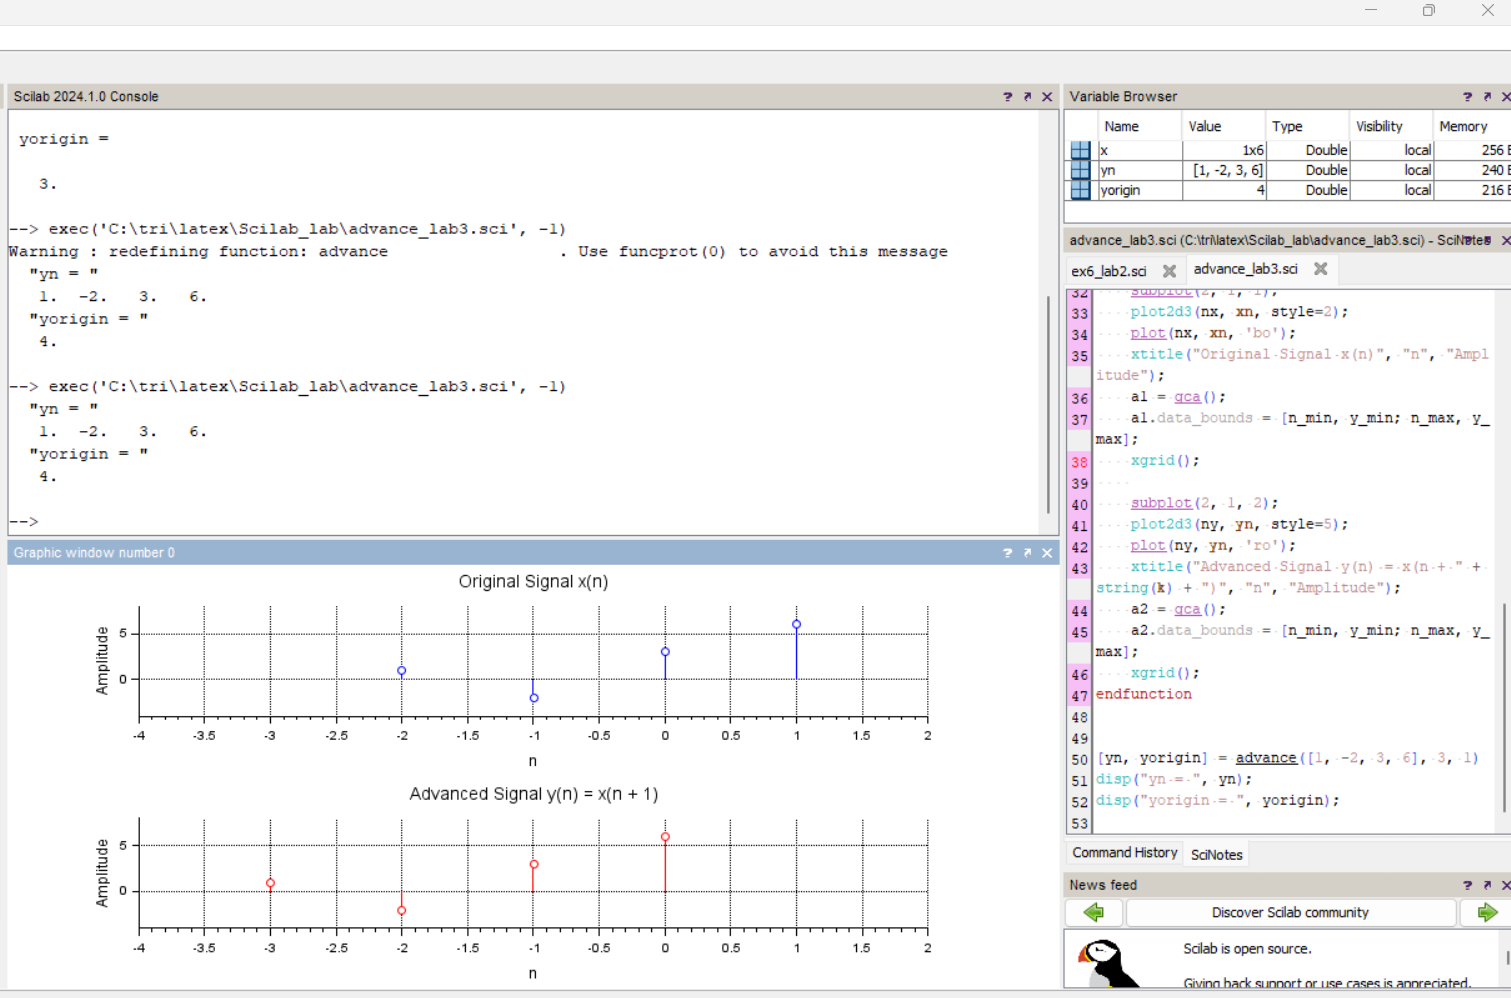
\includegraphics[width=\textwidth]{figures/lap3_advance.png}
    \caption{Result of Exercise 2 -- \texttt{advance([1, -2, 3, 6], 3, 1)}: $x(n)$ (top) and $y(n)=x(n+1)$ (bottom)}
\end{figure}
The figure confirms the analysis: all four samples are shifted one unit to the left, and the sample $6$ is now at $n=0$.

% =================================================================
\subsection{Exercise 3 -- Folding}\label{sec:ex3}
% =================================================================
\textbf{Question:} Write the function \texttt{[yn, yorigin] = fold(xn, xorigin)} that performs the folding operation $y(n) = x(-n)$. $x(n)$ and $y(n)$ are graphically displayed in the same figure.

\textbf{Explanation:}
\writespace[3.5cm]{Explanation of the folding algorithm.}

\textbf{Source code:}
% \scilabfile{src/fold_lab3.sci}{Function \texttt{fold}}
\writespace[6cm]{Source code of \texttt{fold\_lab3.sci}.}

\textbf{Result:}
% \begin{figure}[H]
%     \centering
%     \includegraphics[width=\textwidth]{figures/lap3_fold.png}
%     \caption{Result of Exercise 3 -- \texttt{fold}}
% \end{figure}
\writespace[7cm]{Screenshot of the console output and the figure of $x(n)$ and $y(n)$.}

% =================================================================
\subsection{Exercise 4 -- Addition}\label{sec:ex4}
% =================================================================
\textbf{Question:} Write the function \texttt{[yn, yorigin] = add(x1n, x1origin, x2n, x2origin)} that performs the addition $y(n) = x_1(n) + x_2(n)$. $x_1(n)$, $x_2(n)$ and $y(n)$ are graphically displayed in the same figure.

For example, with $x_1(n) = \{\org{0}, 1, 3, -2\}$ and $x_2(n) = \{1, \org{1}, 2, 3\}$, the call \texttt{[yn, yorigin] = add([0, 1, 3, -2], 1, [1, 1, 2, 3], 2)} must return \texttt{yn = [1, 1, 3, 6, -2]} and \texttt{yorigin = 2}.

\textbf{Explanation:}
Signals are added \emph{sample by sample at the same time index}, not element by element in the vectors. If the two vectors have different lengths or different origins, they cannot be added directly with \texttt{+}. The function works in four steps:
\begin{enumerate}
    \item Build the index vectors $n_1$ and $n_2$ of the two signals using \eqref{eq:index}.
    \item Find the common time range that covers both signals:
    \begin{equation}
        n_{min} = \min(n_{1,min}, n_{2,min}), \qquad n_{max} = \max(n_{1,max}, n_{2,max}).
    \end{equation}
    The origin of the output is at position $\texttt{yorigin} = 1 - n_{min}$.
    \item Zero-pad each signal on the left with $(n_{i,min} - n_{min})$ zeros and on the right with $(n_{max} - n_{i,max})$ zeros. After padding, both vectors have the same length and position $i$ refers to the same time index in both.
    \item Add the two padded vectors element-wise: \texttt{yn = x1\_pad + x2\_pad}.
\end{enumerate}
For the example, $n_1 \in [0, 3]$ and $n_2 \in [-1, 2]$, so the common range is $[-1, 3]$:
\begin{center}
\begin{tabular}{|c|c|c|c|c|c|}
    \hline
    \rowcolor{headergray} $n$ & $-1$ & $0$ & $1$ & $2$ & $3$ \\ \hline
    $x_1(n)$ & 0 & 0 & 1 & 3 & $-2$ \\ \hline
    $x_2(n)$ & 1 & 1 & 2 & 3 & 0 \\ \hline
    $y(n)$   & \textbf{1} & \textbf{1} & \textbf{3} & \textbf{6} & $\mathbf{-2}$ \\ \hline
\end{tabular}
\end{center}
\begin{equation}
    y(n) = \{1, \org{1}, 3, 6, -2\}, \qquad \texttt{yn} = [1, 1, 3, 6, -2], \quad \texttt{yorigin} = 1 - (-1) = 2,
\end{equation}
which matches the expected output given in the assignment.

\textbf{Source code:}
\scilabfile{src/add_lap3.sci}{Function \texttt{add} (\texttt{add\_lap3.sci})}

\textbf{Result:}
\begin{consoleoutput}[Console output]
yn = \\
\quad 1. \quad 1. \quad 3. \quad 6. \quad -2.\\
yorigin = \\
\quad 2.
\end{consoleoutput}

\begin{figure}[H]
    \centering
    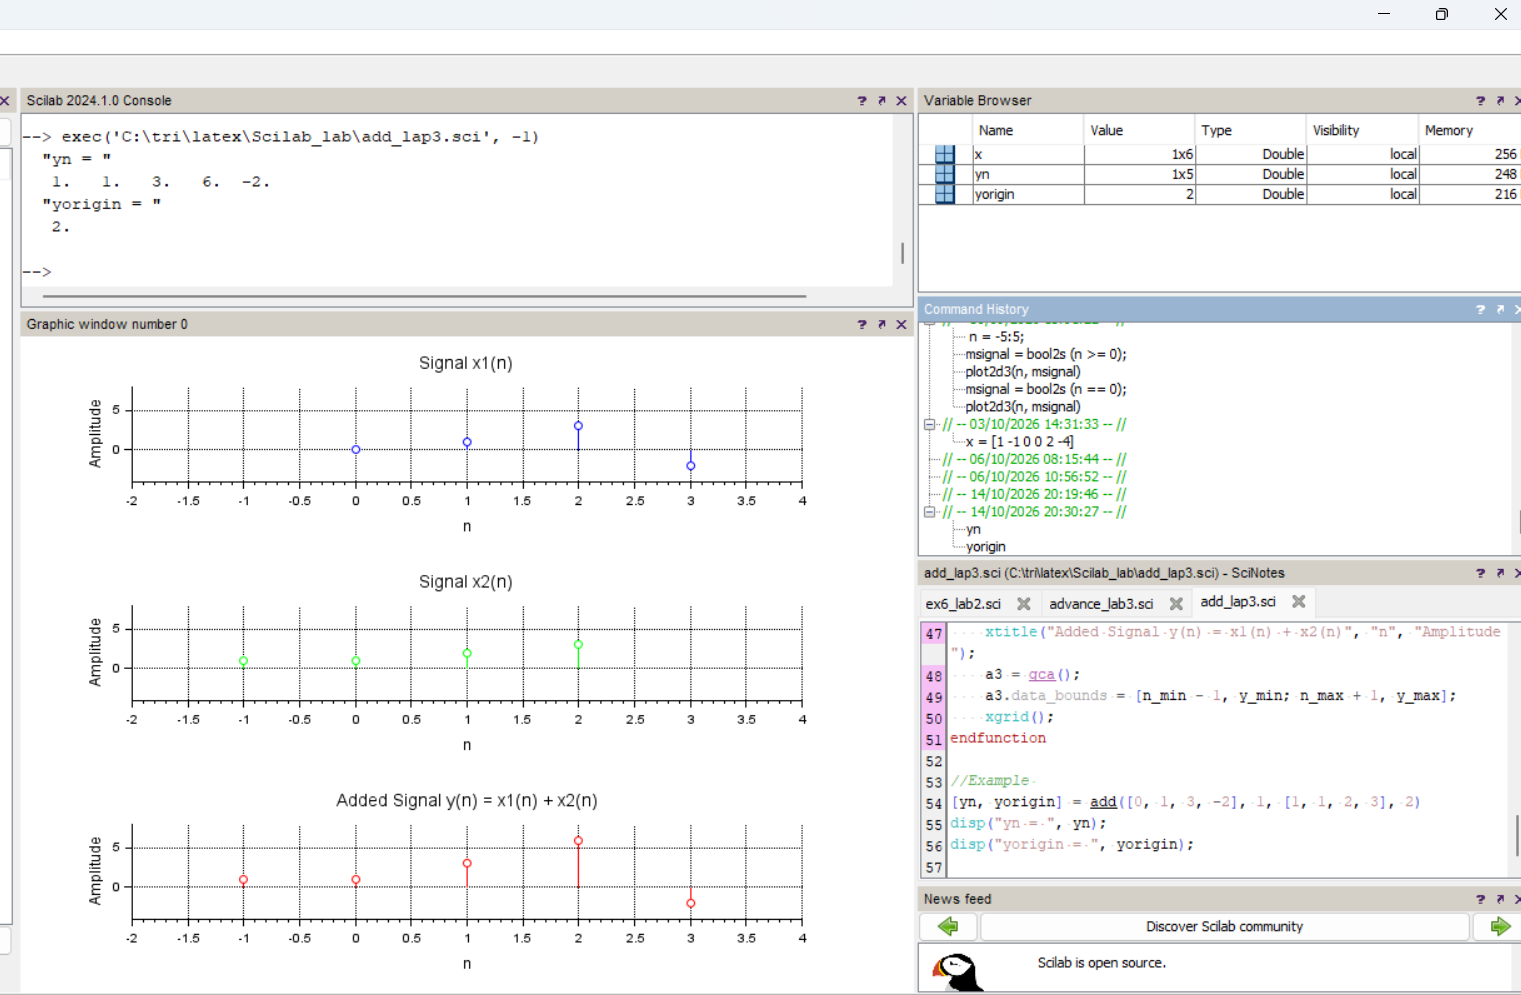
\includegraphics[width=\textwidth]{figures/lap3_add.png}
    \caption{Result of Exercise 4 -- \texttt{add([0, 1, 3, -2], 1, [1, 1, 2, 3], 2)}: $x_1(n)$, $x_2(n)$ and $y(n)=x_1(n)+x_2(n)$}
\end{figure}

% =================================================================
\subsection{Exercise 5 -- Multiplication}\label{sec:ex5}
% =================================================================
\textbf{Question:} Write the function \texttt{[yn, yorigin] = multi(x1n, x1origin, x2n, x2origin)} that performs the multiplication $y(n) = x_1(n)\cdot x_2(n)$. $x_1(n)$, $x_2(n)$ and $y(n)$ are graphically displayed in the same figure.

\textbf{Explanation:}
\writespace[3.5cm]{Explanation of the multiplication algorithm.}

\textbf{Source code:}
% \scilabfile{src/multi_lab3.sci}{Function \texttt{multi}}
\writespace[6cm]{Source code of \texttt{multi\_lab3.sci}.}

\textbf{Result:}
% \begin{figure}[H]
%     \centering
%     \includegraphics[width=\textwidth]{figures/lap3_multi.png}
%     \caption{Result of Exercise 5 -- \texttt{multi}}
% \end{figure}
\writespace[7cm]{Screenshot of the console output and the figure of $x_1(n)$, $x_2(n)$ and $y(n)$.}

% =================================================================
\subsection{Exercise 6 -- Convolution}\label{sec:ex6}
% =================================================================
\textbf{Question:} Write the function \texttt{[yn, yorigin] = convolution(xn, xorigin, hn, horigin)} that performs the convolution $y(n) = x(n) * h(n)$, where $x(n)$ is the input signal and $h(n)$ is the impulse response of the system.

\textbf{Explanation:}
The output of an LTI system is the convolution sum of the input and the impulse response:
\begin{equation}
    y(n) = x(n) * h(n) = \sum_{k=-\infty}^{\infty} x(k)\,h(n-k).
\end{equation}
\begin{itemize}
    \item \textbf{Sample values.} For finite sequences, the convolution sum is the same as multiplying two polynomials. Scilab computes it directly with \texttt{conv(xn, hn)}. If $x(n)$ has $N$ samples and $h(n)$ has $M$ samples, $y(n)$ has $N+M-1$ samples.
    \item \textbf{Origin.} The first sample of $y(n)$ is at the sum of the first indices of the two inputs:
    \begin{equation}
        n_{y,min} = n_{x,min} + n_{h,min} = (1-\texttt{xorigin}) + (1-\texttt{horigin}),
    \end{equation}
    so the origin of $y(n)$ is at position
    \begin{equation}
        \texttt{yorigin} = 1 - n_{y,min} = \texttt{xorigin} + \texttt{horigin} - 1 .
    \end{equation}
\end{itemize}
\textbf{Example:} $x(n) = \{1, \org{2}, 3, 1\}$ (\texttt{xorigin = 2}) and $h(n) = \{\org{1}, 2, 1, -1\}$ (\texttt{horigin = 1}). The output starts at $n = -1 + 0 = -1$ and has $4 + 4 - 1 = 7$ samples. Computing the convolution sum by hand:
\begin{align*}
    y(-1) &= x(-1)h(0) = 1\\
    y(0)  &= x(-1)h(1) + x(0)h(0) = 2 + 2 = 4\\
    y(1)  &= x(-1)h(2) + x(0)h(1) + x(1)h(0) = 1 + 4 + 3 = 8\\
    y(2)  &= x(-1)h(3) + x(0)h(2) + x(1)h(1) + x(2)h(0) = -1 + 2 + 6 + 1 = 8\\
    y(3)  &= x(0)h(3) + x(1)h(2) + x(2)h(1) = -2 + 3 + 2 = 3\\
    y(4)  &= x(1)h(3) + x(2)h(2) = -3 + 1 = -2\\
    y(5)  &= x(2)h(3) = -1
\end{align*}
\begin{equation}
    y(n) = \{1, \org{4}, 8, 8, 3, -2, -1\}, \qquad \texttt{yorigin} = 2 + 1 - 1 = 2 .
\end{equation}

\textbf{Source code:}
\scilabfile{src/convolution_lap3.sci}{Function \texttt{convolution} (\texttt{convolution\_lap3.sci})}

\textbf{Result:}
\begin{consoleoutput}[Console output]
yn = \\
\quad 1. \quad 4. \quad 8. \quad 8. \quad 3. \quad -2. \quad -1.\\
yorigin = \\
\quad 2.
\end{consoleoutput}

\begin{figure}[H]
    \centering
    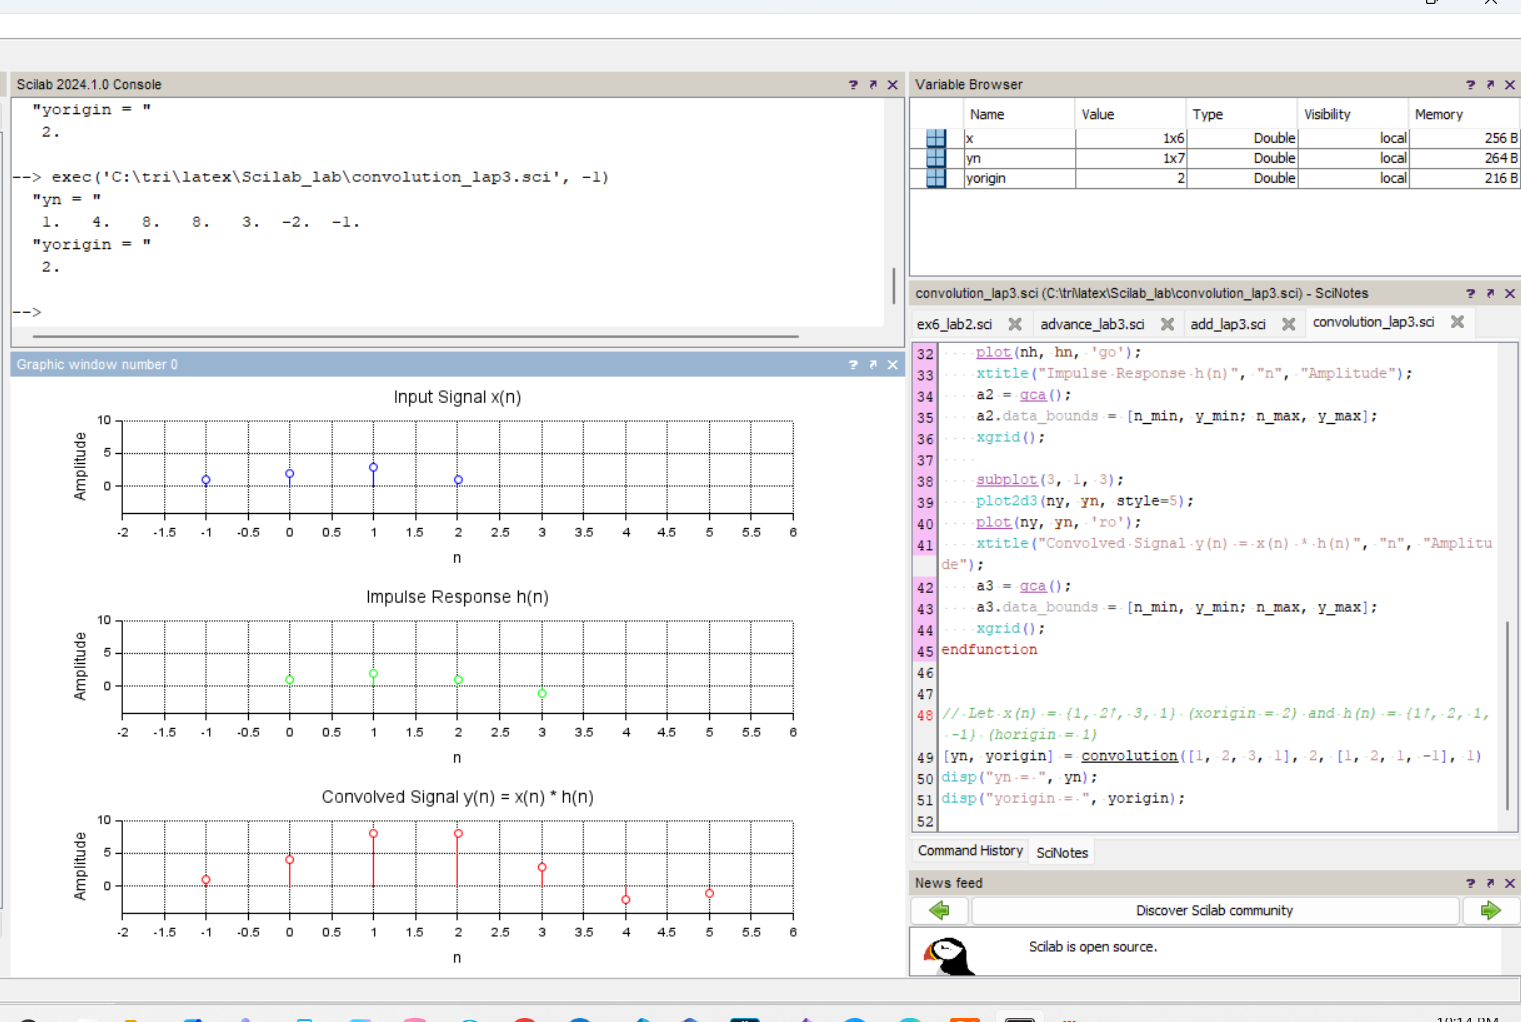
\includegraphics[width=\textwidth]{figures/convolution_lap3.png}
    \caption{Result of Exercise 6 -- \texttt{convolution([1, 2, 3, 1], 2, [1, 2, 1, -1], 1)}: $x(n)$, $h(n)$ and $y(n)=x(n)*h(n)$}
\end{figure}
The Scilab result matches the hand calculation exactly.

% =================================================================
\subsection{Additional Exercises}
% =================================================================

% -----------------------------------------------------------------
\subsubsection*{Additional exercise 2.1}\label{sec:a21}
\addcontentsline{toc}{subsubsection}{Additional exercise 2.1}
% -----------------------------------------------------------------
\noindent A discrete-time signal $x(n)$ is defined as
\[
x(n) = \begin{cases}
    1 + \dfrac{n}{3}, & -3 \le n \le -1\\[4pt]
    1, & 0 \le n \le 3\\
    0, & \text{elsewhere}
\end{cases}
\]
\begin{enumerate}[label=\textbf{(\alph*)}, leftmargin=*]
    \item Determine its values and sketch the signal $x(n)$.
    \item Sketch the signals that result if we:
    \begin{enumerate}[label=\arabic*.]
        \item First fold $x(n)$ and then delay the resulting signal by four samples.
        \item First delay $x(n)$ by four samples and then fold the resulting signal.
    \end{enumerate}
    \item Sketch the signal $x(-n+4)$.
    \item Compare the results in parts (b) and (c) and derive a rule for obtaining the signal $x(-n+k)$ from $x(n)$.
    \item Can you express the signal $x(n)$ in terms of signals $\delta(n)$ and $u(n)$?
\end{enumerate}

\noindent\textbf{Answer:}
\begin{enumerate}[label=\textbf{(\alph*)}, leftmargin=*]
    \item \writespace[3cm]{Answer (a)}
    \item \writespace[4cm]{Answer (b)}
    \item \writespace[3cm]{Answer (c)}
    \item \writespace[3cm]{Answer (d)}
    \item \writespace[3cm]{Answer (e)}
\end{enumerate}

\noindent\textbf{Scilab:}
\writespace[5cm]{Scilab source code for exercise 2.1.}
\writespace[7cm]{Scilab output figure for exercise 2.1.}

% -----------------------------------------------------------------
\subsubsection*{Additional exercise 2.2}\label{sec:a22}
\addcontentsline{toc}{subsubsection}{Additional exercise 2.2}
% -----------------------------------------------------------------
\noindent A discrete-time signal $x(n)$ is shown in Fig. P2.2. Sketch and label carefully each of the following signals.

\begin{figure}[H]
    \centering
    \begin{tikzpicture}[x=0.9cm, y=1.6cm]
        \draw[->] (-4.6,0) -- (6.6,0) node[right] {$n$};
        \foreach \n in {-4,-3,-2,5,6} \fill (\n,0) circle (2pt);
        \foreach \n in {-1,0,1,2} {\draw (\n,0) -- (\n,1); \fill (\n,1) circle (2pt); \node[above] at (\n,1) {$1$};}
        \foreach \n in {3,4} {\draw (\n,0) -- (\n,0.5); \fill (\n,0.5) circle (2pt); \node[above] at (\n,0.5) {$\frac{1}{2}$};}
        \foreach \n in {-2,-1,0,1,2,3,4} \node[below] at (\n,0) {\small $\n$};
        \node at (2.5,1.45) {$x(n)$};
    \end{tikzpicture}
    \caption{Figure P2.2 -- the signal $x(n)$}
\end{figure}

\noindent\textbf{(a)} $x(n-2)$ \quad \textbf{(b)} $x(4-n)$ \quad \textbf{(c)} $x(n+2)$ \quad \textbf{(d)} $x(n)u(2-n)$ \quad \textbf{(e)} $x(n-1)\delta(n-3)$ \quad \textbf{(f)} $x(n^2)$ \quad \textbf{(g)} even part of $x(n)$ \quad \textbf{(h)} odd part of $x(n)$

\noindent\textbf{Answer:}
From the figure, $x(-1)=x(0)=x(1)=x(2)=1$, $x(3)=x(4)=\frac{1}{2}$ and $x(n)=0$ elsewhere:
\[
x(n) = \{\dots, 0, 1, \org{1}, 1, 1, \tfrac{1}{2}, \tfrac{1}{2}, 0, \dots\}
\]
\begin{enumerate}[label=\textbf{(\alph*)}, leftmargin=*]
    \item $x(n-2)$ is $x(n)$ \emph{delayed} by 2 samples (shifted 2 units to the right). The support moves from $[-1, 4]$ to $[1, 6]$:
    \[ x(n-2) = \{\org{0}, 1, 1, 1, 1, \tfrac{1}{2}, \tfrac{1}{2}\} \]

    \item $x(4-n) = x\big(-(n-4)\big)$: first fold $x(n)$ to get $x(-n) = \{\tfrac12, \tfrac12, 1, 1, \org{1}, 1\}$ (support $[-4, 1]$), then delay the folded signal by 4 samples (support $[0, 5]$):
    \[ x(4-n) = \{\org{\tfrac{1}{2}}, \tfrac{1}{2}, 1, 1, 1, 1\} \]
    Check: $y(0) = x(4) = \frac12$ and $y(5) = x(-1) = 1$.

    \item $x(n+2)$ is $x(n)$ \emph{advanced} by 2 samples (shifted 2 units to the left). The support moves to $[-3, 2]$:
    \[ x(n+2) = \{1, 1, 1, \org{1}, \tfrac{1}{2}, \tfrac{1}{2}\} \]

    \item $u(2-n) = 1$ for $n \le 2$ and $0$ for $n > 2$, so it keeps only the samples with $n \le 2$:
    \[ x(n)u(2-n) = \{1, \org{1}, 1, 1\} \]

    \item $\delta(n-3)$ is non-zero only at $n = 3$, so $x(n-1)\delta(n-3) = x(3-1)\,\delta(n-3) = x(2)\,\delta(n-3) = \delta(n-3)$:
    \[ x(n-1)\delta(n-3) = \{\org{0}, 0, 0, 1\} \]

    \item $x(n^2)$: $n = 0 \Rightarrow x(0) = 1$; $n = \pm1 \Rightarrow x(1) = 1$; $n = \pm 2 \Rightarrow x(4) = \frac12$; $|n| \ge 3 \Rightarrow n^2 \ge 9 \Rightarrow x(n^2) = 0$:
    \[ x(n^2) = \{\tfrac{1}{2}, 1, \org{1}, 1, \tfrac{1}{2}\} \]

    \item[\textbf{(g)(h)}] The even and odd parts are $x_e(n) = \frac{x(n)+x(-n)}{2}$ and $x_o(n) = \frac{x(n)-x(-n)}{2}$:
    \begin{center}
    \begin{tabular}{|c|c|c|c|c|c|c|c|c|c|}
        \hline
        \rowcolor{headergray} $n$ & $-4$ & $-3$ & $-2$ & $-1$ & $0$ & $1$ & $2$ & $3$ & $4$ \\ \hline
        $x(n)$   & 0 & 0 & 0 & 1 & 1 & 1 & 1 & $\frac12$ & $\frac12$ \\ \hline
        $x(-n)$  & $\frac12$ & $\frac12$ & 1 & 1 & 1 & 1 & 0 & 0 & 0 \\ \hline
        $x_e(n)$ & $\frac14$ & $\frac14$ & $\frac12$ & 1 & 1 & 1 & $\frac12$ & $\frac14$ & $\frac14$ \\ \hline
        $x_o(n)$ & $-\frac14$ & $-\frac14$ & $-\frac12$ & 0 & 0 & 0 & $\frac12$ & $\frac14$ & $\frac14$ \\ \hline
    \end{tabular}
    \end{center}
    \[ x_e(n) = \{\tfrac14, \tfrac14, \tfrac12, 1, \org{1}, 1, \tfrac12, \tfrac14, \tfrac14\}, \qquad
       x_o(n) = \{-\tfrac14, -\tfrac14, -\tfrac12, 0, \org{0}, 0, \tfrac12, \tfrac14, \tfrac14\} \]
    We can check that $x_e(n) = x_e(-n)$, $x_o(n) = -x_o(-n)$ and $x_e(n) + x_o(n) = x(n)$.
\end{enumerate}

\noindent\textbf{Scilab:} The signal $x(n)$ is written as a Scilab function \texttt{xsig(n)} that can be evaluated at \emph{any} integer index vector. Each transformation is then obtained just by changing the argument, e.g.\ \texttt{xsig(4 - n)} or \texttt{xsig(n.\^{}2)}, over a common index grid $n = -6, \dots, 8$.

\scilabfile{src/ex2_2_lab3.sce}{Additional exercise 2.2 (\texttt{ex2\_2\_lab3.sce})}

\begin{consoleoutput}[Console output]
\textit{(* marks the sample at $n = 0$)}\\[4pt]
x(n) \hfill = \{1, 1*, 1, 1, 0.5, 0.5\}, \quad $n = -1..4$\\
(a) x(n-2) \hfill = \{0*, 1, 1, 1, 1, 0.5, 0.5\}, \quad $n = 0..6$\\
(b) x(4-n) \hfill = \{0.5*, 0.5, 1, 1, 1, 1\}, \quad $n = 0..5$\\
(c) x(n+2) \hfill = \{1, 1, 1, 1*, 0.5, 0.5\}, \quad $n = -3..2$\\
(d) x(n)u(2-n) \hfill = \{1, 1*, 1, 1\}, \quad $n = -1..2$\\
(e) x(n-1)d(n-3) \hfill = \{0*, 0, 0, 1\}, \quad $n = 0..3$\\
(f) x($n^2$) \hfill = \{0.5, 1, 1*, 1, 0.5\}, \quad $n = -2..2$\\
(g) xe(n) \hfill = \{0.25, 0.25, 0.5, 1, 1*, 1, 0.5, 0.25, 0.25\}, \quad $n = -4..4$\\
(h) xo(n) \hfill = \{-0.25, -0.25, -0.5, 0, 0*, 0, 0.5, 0.25, 0.25\}, \quad $n = -4..4$\\[2pt]
Check xe(n) + xo(n) = x(n): T
\end{consoleoutput}

\begin{figure}[H]
    \centering
    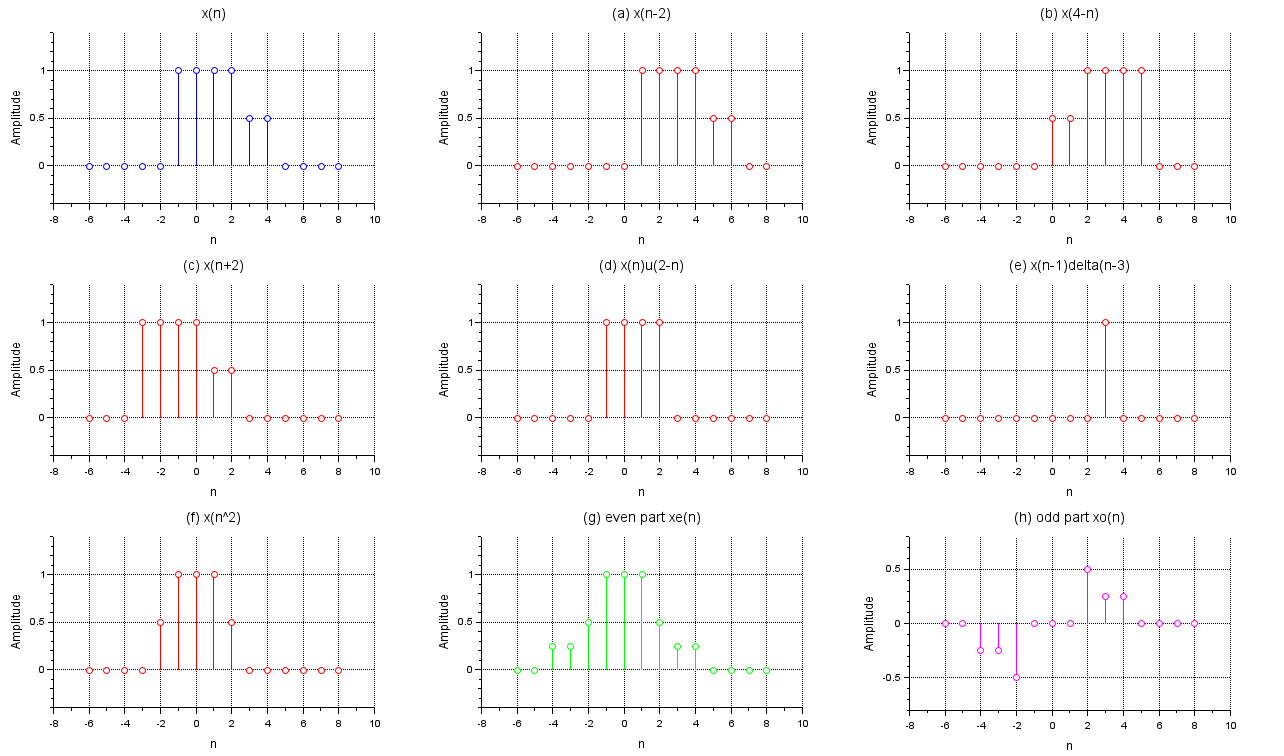
\includegraphics[width=\textwidth]{figures/ex2_2.png}
    \caption{Additional exercise 2.2 -- $x(n)$ and the signals (a)--(h)}
\end{figure}
The Scilab results agree with all the hand-derived sequences (a)--(h).

% -----------------------------------------------------------------
\subsubsection*{Additional exercise 2.4}\label{sec:a24}
\addcontentsline{toc}{subsubsection}{Additional exercise 2.4}
% -----------------------------------------------------------------
\noindent Show that any signal can be decomposed into an even and an odd component. Is the decomposition unique? Illustrate your arguments using the signal
\[ x(n) = \{2, 3, \org{4}, 5, 6\} \]

\noindent\textbf{Answer:}

\noindent\textbf{Existence.} For any signal $x(n)$, define
\begin{equation}
    x_e(n) = \frac{1}{2}\big[x(n) + x(-n)\big], \qquad x_o(n) = \frac{1}{2}\big[x(n) - x(-n)\big].
\end{equation}
Then
\begin{itemize}
    \item $x_e(-n) = \frac12\big[x(-n) + x(n)\big] = x_e(n)$, so $x_e(n)$ is \textbf{even};
    \item $x_o(-n) = \frac12\big[x(-n) - x(n)\big] = -x_o(n)$, so $x_o(n)$ is \textbf{odd};
    \item $x_e(n) + x_o(n) = \frac12 x(n) + \frac12 x(-n) + \frac12 x(n) - \frac12 x(-n) = x(n)$.
\end{itemize}
Hence every signal can be written as the sum of an even and an odd component.

\noindent\textbf{Uniqueness.} Suppose $x(n) = e(n) + o(n)$ for \emph{some} even signal $e(n)$ and \emph{some} odd signal $o(n)$. Replacing $n$ by $-n$ and using $e(-n) = e(n)$, $o(-n) = -o(n)$:
\[
\begin{cases}
    x(n)  = e(n) + o(n)\\
    x(-n) = e(n) - o(n)
\end{cases}
\;\Longrightarrow\;
e(n) = \frac{x(n)+x(-n)}{2} = x_e(n), \quad o(n) = \frac{x(n)-x(-n)}{2} = x_o(n).
\]
Any even/odd pair that adds up to $x(n)$ must equal $x_e(n)$ and $x_o(n)$, so \textbf{the decomposition is unique}.

\noindent\textbf{Illustration.} With $x(n) = \{2, 3, \org{4}, 5, 6\}$ we have $x(-n) = \{6, 5, \org{4}, 3, 2\}$:
\begin{center}
\begin{tabular}{|c|c|c|c|c|c|}
    \hline
    \rowcolor{headergray} $n$ & $-2$ & $-1$ & $0$ & $1$ & $2$ \\ \hline
    $x(n)$   & 2 & 3 & 4 & 5 & 6 \\ \hline
    $x(-n)$  & 6 & 5 & 4 & 3 & 2 \\ \hline
    $x_e(n)$ & 4 & 4 & 4 & 4 & 4 \\ \hline
    $x_o(n)$ & $-2$ & $-1$ & 0 & 1 & 2 \\ \hline
\end{tabular}
\end{center}
\[ x_e(n) = \{4, 4, \org{4}, 4, 4\}, \qquad x_o(n) = \{-2, -1, \org{0}, 1, 2\} \]
$x_e(n)$ is symmetric about $n = 0$, $x_o(n)$ is anti-symmetric with $x_o(0)=0$, and their sum gives back $\{2, 3, \org{4}, 5, 6\}$. For example, the split $\{2,3,\org{4},5,6\} = \{2,3,\org{4},3,2\} + \{0,0,\org{0},2,4\}$ also sums to $x(n)$, but the second part is not odd. By the uniqueness proof, no other even/odd pair is possible.

\noindent\textbf{Scilab:} The function \texttt{evenodd(xn, xorigin)} uses the same (vector, origin) convention as the lab functions. It places $x(n)$ on a symmetric grid $[-L, L]$, so folding is just reversing the vector (\texttt{xs(\$:-1:1)}).

\scilabfile{src/ex2_4_lab3.sce}{Additional exercise 2.4 (\texttt{ex2\_4\_lab3.sce})}

\begin{consoleoutput}[Console output]
n \qquad\quad = -2 \quad -1 \quad 0 \quad 1 \quad 2\\
x(n) \quad\ \ = 2 \quad 3 \quad 4 \quad 5 \quad 6\\
x(-n) \quad = 6 \quad 5 \quad 4 \quad 3 \quad 2\\
xe(n) \quad = 4 \quad 4 \quad 4 \quad 4 \quad 4\\
xo(n) \quad = -2 \quad -1 \quad 0 \quad 1 \quad 2\\
yorigin = 3\\
xe even  (xe(n) =  xe(-n)) : T\\
xo odd   (xo(n) = -xo(-n)) : T\\
xe + xo == x \qquad\qquad\quad\ : T
\end{consoleoutput}

\begin{figure}[H]
    \centering
    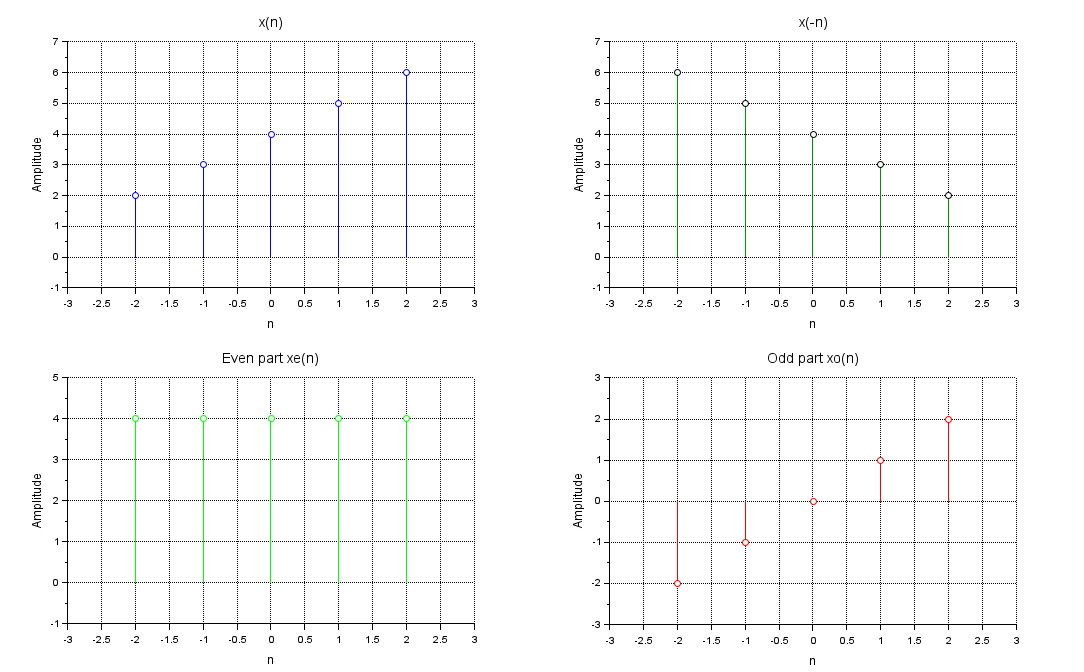
\includegraphics[width=0.9\textwidth]{figures/ex2_4.png}
    \caption{Additional exercise 2.4 -- $x(n)$, $x(-n)$, even part $x_e(n)$ and odd part $x_o(n)$}
\end{figure}

% -----------------------------------------------------------------
\subsubsection*{Additional exercise 2.6}\label{sec:a26}
\addcontentsline{toc}{subsubsection}{Additional exercise 2.6}
% -----------------------------------------------------------------
\noindent Consider the system $y(n) = \mathcal{T}[x(n)] = x(n^2)$.
\begin{enumerate}[label=\textbf{(\alph*)}, leftmargin=*]
    \item Determine if the system is time invariant.
    \item To clarify the result in part (a) assume that the signal
    $x(n) = \begin{cases} 1, & 0 \le n \le 3\\ 0, & \text{elsewhere}\end{cases}$
    is applied into the system.
    (1) Sketch the signal $x(n)$.
    (2) Determine and sketch the signal $y(n) = \mathcal{T}[x(n)]$.
    (3) Sketch the signal $y_2'(n) = y(n-2)$.
    (4) Determine and sketch the signal $x_2(n) = x(n-2)$.
    (5) Determine and sketch the signal $y_2(n) = \mathcal{T}[x_2(n)]$.
    (6) Compare the signals $y_2(n)$ and $y(n-2)$. What is your conclusion?
    \item Repeat part (b) for the system $y(n) = x(n) - x(n-1)$. Can you use this result to make any statement about the time invariance of this system? Why?
    \item Repeat parts (b) and (c) for the system $y(n) = \mathcal{T}[x(n)] = n\,x(n)$.
\end{enumerate}

\noindent\textbf{Answer:}

A system is \textbf{time invariant} if shifting the input by $k$ only shifts the output by the same $k$:
\[ x(n) \xrightarrow{\ \mathcal{T}\ } y(n) \quad \Longrightarrow \quad x(n-k) \xrightarrow{\ \mathcal{T}\ } y(n-k), \quad \forall\, x(n), \forall\, k. \]

\begin{enumerate}[label=\textbf{(\alph*)}, leftmargin=*]
    \item For $y(n) = x(n^2)$, the response to the delayed input $x(n-k)$ is obtained by replacing $n$ by $n^2$ \emph{inside the argument of the input only}:
    \[ y(n,k) = \mathcal{T}[x(n-k)] = x(n^2 - k), \]
    while the delayed output is
    \[ y(n-k) = x\big((n-k)^2\big) = x(n^2 - 2nk + k^2). \]
    Since $x(n^2-k) \ne x\big((n-k)^2\big)$ in general, the system is \textbf{time variant}.

    \item With $x(n) = \{\org{1}, 1, 1, 1\}$:
    \begin{enumerate}[label=(\arabic*)]
        \item $x(n) = \{\org{1}, 1, 1, 1\}$, $0 \le n \le 3$.
        \item $y(n) = x(n^2)$: $y(0) = x(0) = 1$, $y(\pm1) = x(1) = 1$, $y(\pm2) = x(4) = 0$, so
        \[ y(n) = \{1, \org{1}, 1\} \]
        \item $y_2'(n) = y(n-2) = \{\org{0}, 1, 1, 1\}$ (non-zero for $1 \le n \le 3$).
        \item $x_2(n) = x(n-2) = \{\org{0}, 0, 1, 1, 1, 1\}$ (non-zero for $2 \le n \le 5$).
        \item $y_2(n) = x_2(n^2) = x(n^2 - 2)$, which equals 1 only when $0 \le n^2 - 2 \le 3 \Leftrightarrow 2 \le n^2 \le 5 \Leftrightarrow n = \pm 2$:
        \[ y_2(n) = \{1, 0, \org{0}, 0, 1\} \]
        \item $y_2(n) = \{1, 0, \org{0}, 0, 1\} \neq y(n-2) = \{\org{0}, 1, 1, 1\}$. One counter-example is enough to show that the system is \textbf{time variant}, which confirms part (a).
    \end{enumerate}

    \item System $y(n) = x(n) - x(n-1)$:
    \begin{enumerate}[label=(\arabic*)]
        \item $x(n) = \{\org{1}, 1, 1, 1\}$.
        \item $y(n) = x(n) - x(n-1) = \{\org{1}, 0, 0, 0, -1\}$ ($y(0) = 1 - 0$, $y(4) = 0 - 1$).
        \item $y(n-2) = \{\org{0}, 0, 1, 0, 0, 0, -1\}$ (non-zero at $n = 2$ and $n = 6$).
        \item $x_2(n) = x(n-2) = \{\org{0}, 0, 1, 1, 1, 1\}$.
        \item $y_2(n) = x_2(n) - x_2(n-1) = \{\org{0}, 0, 1, 0, 0, 0, -1\}$.
        \item $y_2(n) = y(n-2)$ for this input.
    \end{enumerate}
    \textbf{Can we conclude time invariance from this result?} \emph{No.} Time invariance must hold for \emph{every} input and \emph{every} shift $k$. One example where $y_2(n) = y(n-2)$ is consistent with time invariance but does not prove it. (A single counter-example, on the other hand, is enough to prove time \emph{variance}.) To prove it we need the general argument:
    \[ \mathcal{T}[x(n-k)] = x(n-k) - x(n-k-1) = y(n-k) \quad \forall\, x, k, \]
    so the system $y(n) = x(n) - x(n-1)$ is indeed \textbf{time invariant}.

    \item System $y(n) = n\,x(n)$:
    \begin{enumerate}[label=(\arabic*)]
        \item $x(n) = \{\org{1}, 1, 1, 1\}$.
        \item $y(n) = n\,x(n) = \{\org{0}, 1, 2, 3\}$.
        \item $y(n-2) = (n-2)\,x(n-2) = \{\org{0}, 0, 0, 1, 2, 3\}$ (values $0,1,2,3$ at $n = 2,\dots,5$).
        \item $x_2(n) = x(n-2) = \{\org{0}, 0, 1, 1, 1, 1\}$.
        \item $y_2(n) = n\,x_2(n) = \{\org{0}, 0, 2, 3, 4, 5\}$.
        \item $y_2(n) \neq y(n-2)$ (e.g.\ $y_2(2) = 2$ but $y(0) = 0$), so the system is \textbf{time variant}.
    \end{enumerate}
    \textbf{Statement about time invariance (part (c) for this system):} here the example \emph{is} enough to decide, because one counter-example proves time variance. In general,
    \[ \mathcal{T}[x(n-k)] = n\,x(n-k) \;\neq\; y(n-k) = (n-k)\,x(n-k). \]
    The gain $n$ depends explicitly on time, so the system is time variant.
\end{enumerate}

\begin{table}[H]
    \centering
    \caption{Summary of Additional exercise 2.6}
    \begin{tabular}{|l|c|c|}
        \hline
        \rowcolor{headergray}\textbf{System} & $y_2(n)$ vs.\ $y(n-2)$ & \textbf{Conclusion} \\ \hline
        $y(n) = x(n^2)$        & different & Time variant \\ \hline
        $y(n) = x(n) - x(n-1)$ & equal     & Time invariant (proved analytically) \\ \hline
        $y(n) = n\,x(n)$       & different & Time variant \\ \hline
    \end{tabular}
\end{table}

\noindent\textbf{Scilab:} Each system is written as a function \texttt{T(f, n)} that receives the \emph{input signal as a function} \texttt{f} and returns the output at the indices \texttt{n}. This way, $y(n-2)$ is simply \texttt{T(xin, n-2)} and $y_2(n) = \mathcal{T}[x(n-2)]$ is \texttt{T(x2in, n)}. The function \texttt{check\_system} performs steps (1)--(6) for each system. Step (6) is plotted as the difference $y_2(n) - y(n-2)$: if it is identically zero, the shift of the input only shifts the output.

\scilabfile{src/ex2_6_lab3.sce}{Additional exercise 2.6 (\texttt{ex2\_6\_lab3.sce})}

\begin{consoleoutput}[Console output]
\textit{(* marks the sample at $n = 0$)}\\[4pt]
\textbf{----- System 1: $y(n) = x(n^2)$ -----}\\
\ \ x(n) \qquad\quad = \{1*, 1, 1, 1\}, \quad $n = 0..3$\\
\ \ y(n) \qquad\quad = \{1, 1*, 1\}, \quad $n = -1..1$\\
\ \ y(n-2) \qquad = \{0*, 1, 1, 1\}, \quad $n = 0..3$\\
\ \ x2(n)=x(n-2) = \{0*, 0, 1, 1, 1, 1\}, \quad $n = 0..5$\\
\ \ y2(n)=T[x2] \ = \{1, 0, 0*, 0, 1\}, \quad $n = -2..2$\\
\ \ $\Rightarrow$ y2(n) $\neq$ y(n-2) $\Longrightarrow$ \textbf{the system is TIME-VARIANT}\\[4pt]
\textbf{----- System 2: $y(n) = x(n) - x(n-1)$ -----}\\
\ \ x(n) \qquad\quad = \{1*, 1, 1, 1\}, \quad $n = 0..3$\\
\ \ y(n) \qquad\quad = \{1*, 0, 0, 0, -1\}, \quad $n = 0..4$\\
\ \ y(n-2) \qquad = \{0*, 0, 1, 0, 0, 0, -1\}, \quad $n = 0..6$\\
\ \ x2(n)=x(n-2) = \{0*, 0, 1, 1, 1, 1\}, \quad $n = 0..5$\\
\ \ y2(n)=T[x2] \ = \{0*, 0, 1, 0, 0, 0, -1\}, \quad $n = 0..6$\\
\ \ $\Rightarrow$ y2(n) = y(n-2) for this input (consistent with time-invariance)\\[4pt]
\textbf{----- System 3: $y(n) = n\,x(n)$ -----}\\
\ \ x(n) \qquad\quad = \{1*, 1, 1, 1\}, \quad $n = 0..3$\\
\ \ y(n) \qquad\quad = \{0*, 1, 2, 3\}, \quad $n = 0..3$\\
\ \ y(n-2) \qquad = \{0*, 0, 0, 1, 2, 3\}, \quad $n = 0..5$\\
\ \ x2(n)=x(n-2) = \{0*, 0, 1, 1, 1, 1\}, \quad $n = 0..5$\\
\ \ y2(n)=T[x2] \ = \{0*, 0, 2, 3, 4, 5\}, \quad $n = 0..5$\\
\ \ $\Rightarrow$ y2(n) $\neq$ y(n-2) $\Longrightarrow$ \textbf{the system is TIME-VARIANT}
\end{consoleoutput}

\begin{figure}[H]
    \centering
    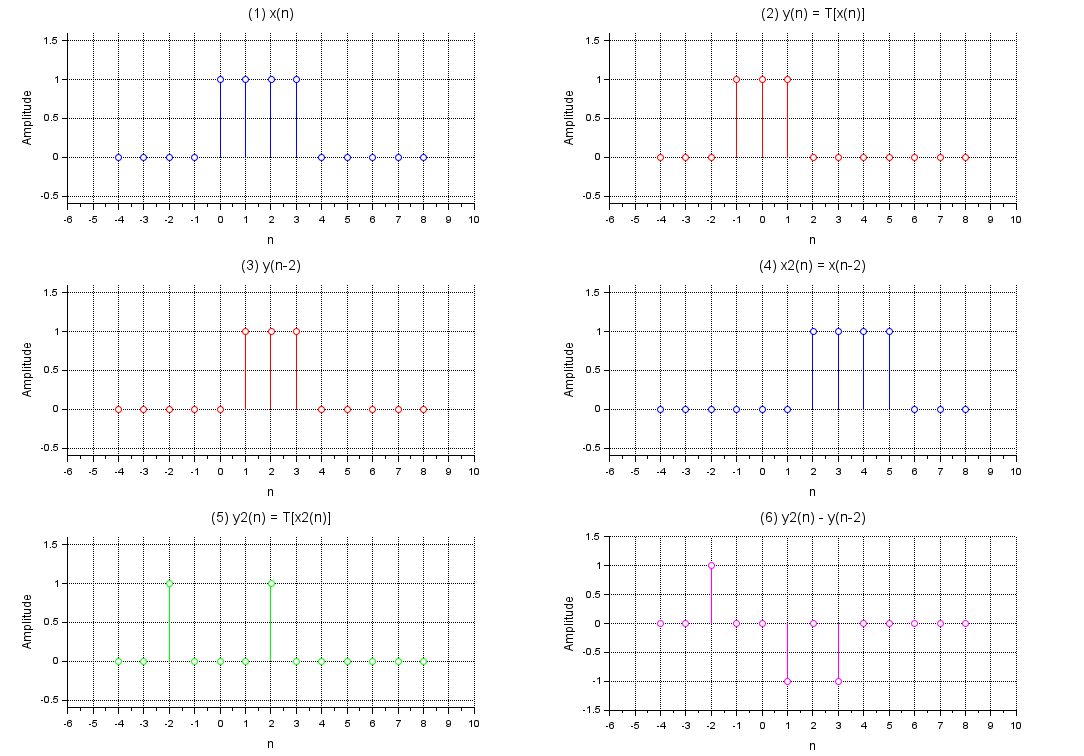
\includegraphics[width=0.9\textwidth]{figures/ex2_6_sys1.png}
    \caption{Additional exercise 2.6(b) -- system $y(n) = x(n^2)$: $y_2(n) - y(n-2) \neq 0$ $\Rightarrow$ time variant}
\end{figure}
\begin{figure}[H]
    \centering
    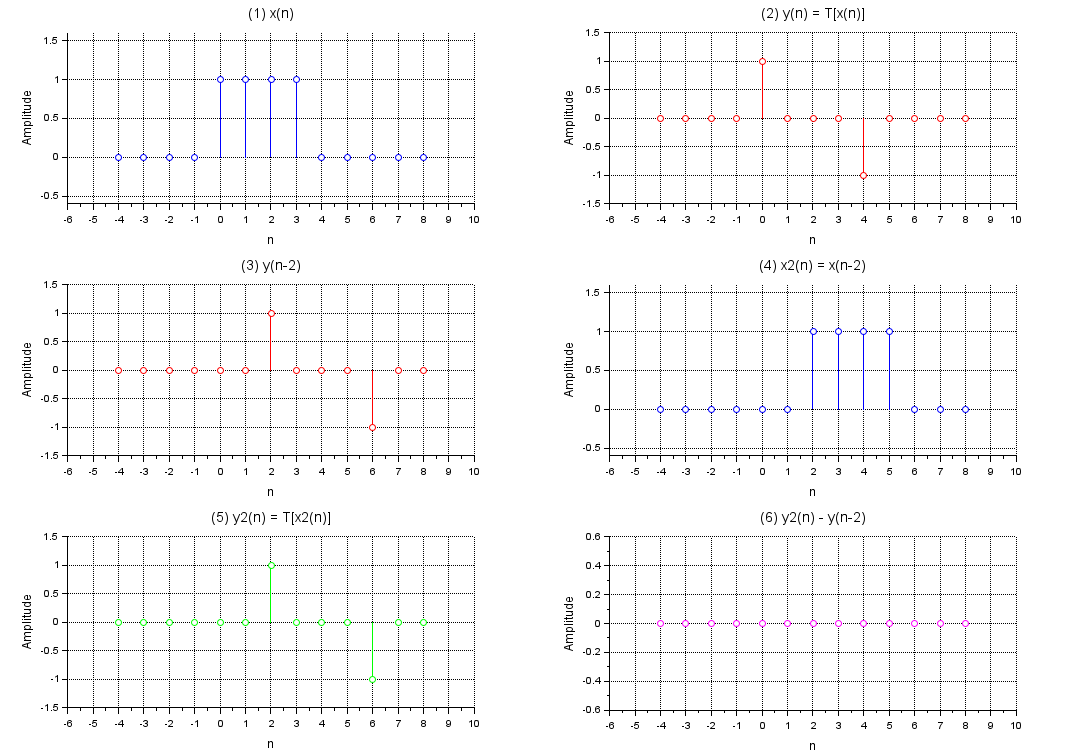
\includegraphics[width=0.9\textwidth]{figures/ex2_6_sys2.png}
    \caption{Additional exercise 2.6(c) -- system $y(n) = x(n) - x(n-1)$: $y_2(n) - y(n-2) = 0$}
\end{figure}
\begin{figure}[H]
    \centering
    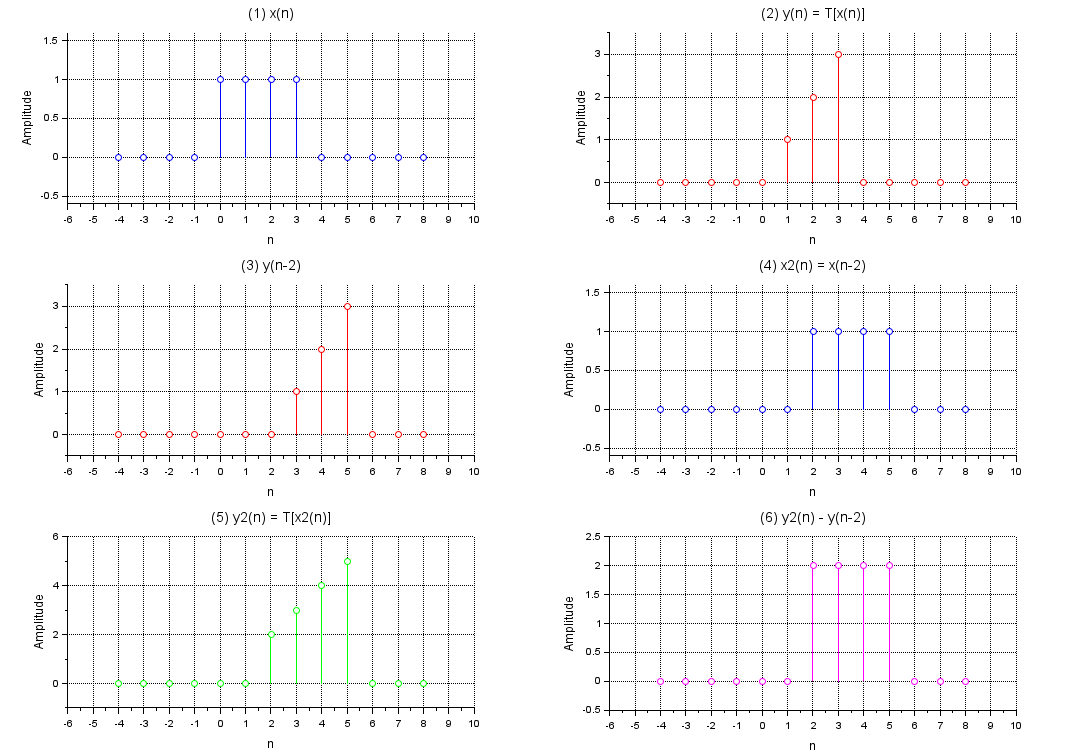
\includegraphics[width=0.9\textwidth]{figures/ex2_6_sys3.png}
    \caption{Additional exercise 2.6(d) -- system $y(n) = n\,x(n)$: $y_2(n) - y(n-2) \neq 0$ $\Rightarrow$ time variant}
\end{figure}

\section{Discussion}
Representing a signal by the pair (vector, origin) made it possible to implement every time-domain operation as a general Scilab function. The exercises show that most operations only need careful index bookkeeping:
\begin{itemize}
    \item Time shifts (\texttt{advance}, \texttt{delay}) leave the sample vector unchanged and only move the origin. Zero-padding is needed only when the origin falls outside the vector.
    \item Sample-by-sample operations (\texttt{add}, \texttt{multi}) require both signals to be aligned on a common index range by zero-padding before using the element-wise operators.
    \item For \texttt{convolution}, the built-in \texttt{conv} gives the sample values, and the origin follows from $n_{y,min} = n_{x,min} + n_{h,min}$.
\end{itemize}
In the additional exercises, evaluating a signal as a function of an arbitrary index vector turned out to be a convenient way to compute folded, shifted or non-linearly indexed signals such as $x(n^2)$. Exercise 2.6 also shows that one example can only \emph{disprove} time invariance. Proving it requires a general argument.

\section{References}
\begin{itemize}
    \item J. G. Proakis and D. G. Manolakis, \emph{Digital Signal Processing: Principles, Algorithms, and Applications}, 4th ed., Pearson, 2007 -- Chapter 2 Problems.
    \item Digital Signal Processing Lecture Notes - Ho Chi Minh City University of Technology.
    \item Scilab Online Manuals: \url{https://help.scilab.org/doc/5.5.2/en_US/function.html}, \url{https://help.scilab.org/doc/5.5.2/en_US/deff.html}.
\end{itemize}

\section{Source Code}
The source code, scripts, and LaTeX files for this laboratory report can be accessed at our GitHub repository: \\
\url{https://github.com/aulequangtri/signal_scilab}

\end{document}
